\documentclass[a4paper]{report}
\usepackage[T1]{fontenc}
\usepackage[utf8]{inputenc}
\usepackage[english]{babel}
\usepackage{titlesec}
\usepackage{lipsum}
\usepackage{booktabs}
\usepackage{hyperref}
\usepackage{graphicx}
\usepackage{float}
\usepackage{rotating}
\usepackage[dvipsnames]{xcolor}
\usepackage{listings}
\usepackage{alloy-style}
\usepackage[shortlabels]{enumitem}
\usepackage{geometry}
\usepackage{pdflscape}
\usepackage{caption}
\usepackage{soul}
\usepackage{blindtext}
\graphicspath{{./images/}}
\begin{document}

%%The two following lines remove the line "Chapter n" at the beginning of each chapter, before the title
%\titleformat{\chapter}[display]
%  {\normalfont\bfseries}{}{0pt}{\Large}
\titleformat{\chapter}[hang] 
{\normalfont\huge\bfseries}{\thechapter}{1em}{} 

\title{eMSP system requirements}
\author{Federico Bono, Daniele Cipollone}
\date{\today}
\maketitle

\begin{titlepage}
\begin{figure}[t]
\centering
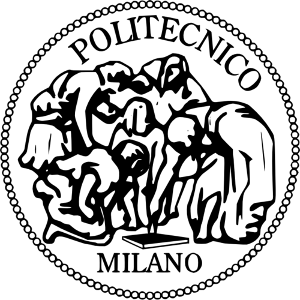
\includegraphics[width=0.3\textwidth]{Logo}
\end{figure}
\begin{center}
    \textsc{ \LARGE{Politecnico di Milano \\}}
	\textsc{ \Large {School of Industrial and Information Engineering\\ }}
	\textnormal{ \Large{Master of Science in Computer Science and Engineering\\}}
	\vspace{3mm}
	\textnormal{ \Large{Software Engineering 2 Project\\}}
	\vspace{30mm}
	\fontsize{10mm}{7mm}\selectfont 
    \textup{eMall - eMSP system}\\
    \textnormal{ \LARGE{Requirement Analysis and Specification Document\\}}
\end{center}

\vspace{18mm}

\begin{center}
    \textnormal{\large{\bf Authors:\\}}
	{\large Federico Bono \\ Daniele Cipollone}
	\fontsize{10mm}{5mm}\selectfont 
\end{center}
\vspace{15mm}

\centering{\large{
Academic Year 2022/2023 \\
\vspace{10mm}
Milano, 06/01/2023 \\
\vspace{2mm}
Version 1.2
}}

\end{titlepage}
\chapter{Introduction}
\section{Purpose}
The purpose of this document is to describe and explain in details the design choices for the development and deployment of the eMSP system of eMall. The description is structured on multiple levels to give an overview of the system from multiple viewpoints. In the following pages you will find:

\begin{enumerate}
	\item High level overview of the architecture
	\item Overview of the components of the system
	\item Deployment overview
	\item Overview of the interactions between components
	\item Overview of the interfaces offered by the various components
	\item The UI of the mobile application used by the final user
	\item The patterns and technologies used in the system
\end{enumerate}

\section{Scope}
eMall App is a platform that helps the end users to plan the charging process, by getting information about Charging Points nearby, their costs and any special offer; book a charge in a specific point, control the charging process and get notified when the charge is completed. It also handles payments for the service.\\\\
In the e-Charging ecosystem, there are many different actors involved that we need to keep into consideration while collecting requirements and designing the system. The first information to consider is that Charging Points are owned and managed by Charging Point Operators (CPOs) and each CPO has its own IT infrastructure, managed via a Charge Point Management System (CPMS). \\\\
In order to comunicate with the various CPMS, the 
\href{../Specs/OCPI-2.2.1.pdf}{OCPI (Open Charge Point Interface) protocol} is used.\\\\
To be able to process payments, the system will need to communicate with a Payment Service Provider (PSP) via the HTTP(s) protocol, using the propertary APIs offered by the provider.\\\\
Given that our system is not the producer of the data, and that there is the need for implementing different functionalities (e.g. payments) a three-tier architecture has been chosen, to separate the data layer (that mostly acts as a cache layer) and the business logic layer.


\section{Definitions, Acronyms, Abbreviations}

\subsection{Definitions}
\begin{tabular}{|p{5cm}|p{10cm}|}
	\hline
	Connector \newline Charging Socket & Physical connector that allow to transfer energy to the connected vehicle\\
	\hline
	Charging slot & Physical device with multiple Connectors that can charge electric vehicles.\newline
	NOTE: from OCPI definitions a Charging Slot can have up to one connector active at any time (i.e. can charge only one Vehicle at any time) \\
	\hline
	Charging Point & Physical structure composed by multiple Charging Slots\\
	\hline
	Maintenance of a charging slot & Activity/activities that results in a momentary unavailability of the charging slot\\
	\hline
	Payment information & information required by the payment provider to be able to charge the user for the service (e.g. credit card number)\\
	\hline
	Charging session & period of time when the vehicle is connected to a charging plug for charging\\
	\hline
	Booking period & period of time between the booking of a charging session and the beginning of the charging session\\
	\hline
	{Guest \newline Guest User} & Unregistered user\\
	\hline
	{User \newline Enabled User \newline Active User} & Registered user with confirmed email and payment method\\
	\hline
	Unconfirmed User & Registered user without confirmed email\\
	\hline
	Pending User & Registered user with confirmed email but no payment method set up\\
	\hline
	Payment Service Provider & External service that provides API to process payments\\
	\hline
\end{tabular}

\subsection{Acronyms}
\begin{tabular}{|l|l|}
	\hline
	eMSP & e-Mobility Service Provider\\
	\hline
	CP & Charge Point / Charging Point\\
	\hline
	CPO & Charging Point Operator\\
	\hline
	CPMS & Charging Point Management System\\
	\hline
	OCPI & Open Charge Point Interface\\
	\hline
	EV & Electric Vehicle\\
	\hline
	PSP & Payment Service Provider\\
	\hline
	API & Application Programming Interface\\
	\hline
\end{tabular}


\section{Revision History}
\begin{itemize}
	\item v1.0 - 05 January 2023
\end{itemize}

\section{Related Documents}
\begin{itemize}
	\item {eMSP RASD (RASD\_eMSP.pdf)}
	\item OCPI specifications document (OCPI-2.2.1.pdf)
\end{itemize}

\section{Document structure}
The document is structured in six sections:

\begin{enumerate}
	\item Description and introduction of the various design choices made during the design of the system. Descriptions are written at different levels of abstractions: from the general point of view to the detailed view of the single component.
	\item User interfaces and design mockups.
	\item The requirement traceability matrix is used to map each component to the requirement(s) that fulfils.
	\item Implementation and test plans for the entire system
	\item Total effort
	\item References used
\end{enumerate}























\chapter{Overall description}
\section{Product perspective}
\subsection{Scenarios}

\begin{enumerate}
	\descitem{User wants to start using the platform}
	Bob has bought a new electric car and wants to start using the eMall network to charge it.\\ Bob goes to the app store to download the official application, opens it and taps on the "Signup" button to initiate the user registration flow. He inserts all the necessary information and, after submitting the form, he's granted access to the system. 
	
	\descitem{User wants to check for charging points availabilities}
	Bob wants to charge his car, he opens the eMall app and, using the integrated map view starts looking for a nearby CPs. After tapping on one of the available Charging Points, the application displays the status of the point, the available charging slots and their connectors as well as the price rates applied.
	
	\descitem{User wants to book a charge for a certain time frame}
	Bob opens the app, searches for an available CP and, after opening the details page, he taps on the "book" button to start the booking process. The application asks for a time frame and a connector type, and after checking for availability, it books the charging slot and returns the booking reference to Bob.
	
	\descitem{User wants to start a charge at the CP}
	Bob goes to a charging point and wants to start charging his vehicle, with a booking for that time frame, he simply needs to park the car in the correct spot, connect it with the correct plug and enable the charge flow via the app. Without a booking, he needs to look for an available spot via the app and start a booking process for it.
	
	\descitem{User wants to be notified at the end of the charge}
	Bob started the charging process a couple of hours ago for a 2 hours time frame. The system checks the booking time-frame and sends a notification to Bob's smartphone with the details of the charging process (e.g. cost and battery status)
	
	\descitem{User wants to pay for the service}
	Bob goes to retrieve his car from the CP, he uses the app to complete the charging process and the system automatically bills his credit card / Paypal account with the required amount.
\end{enumerate}

\newpage

\subsection{Class Diagram}

\begin{figure}[h]
\centering
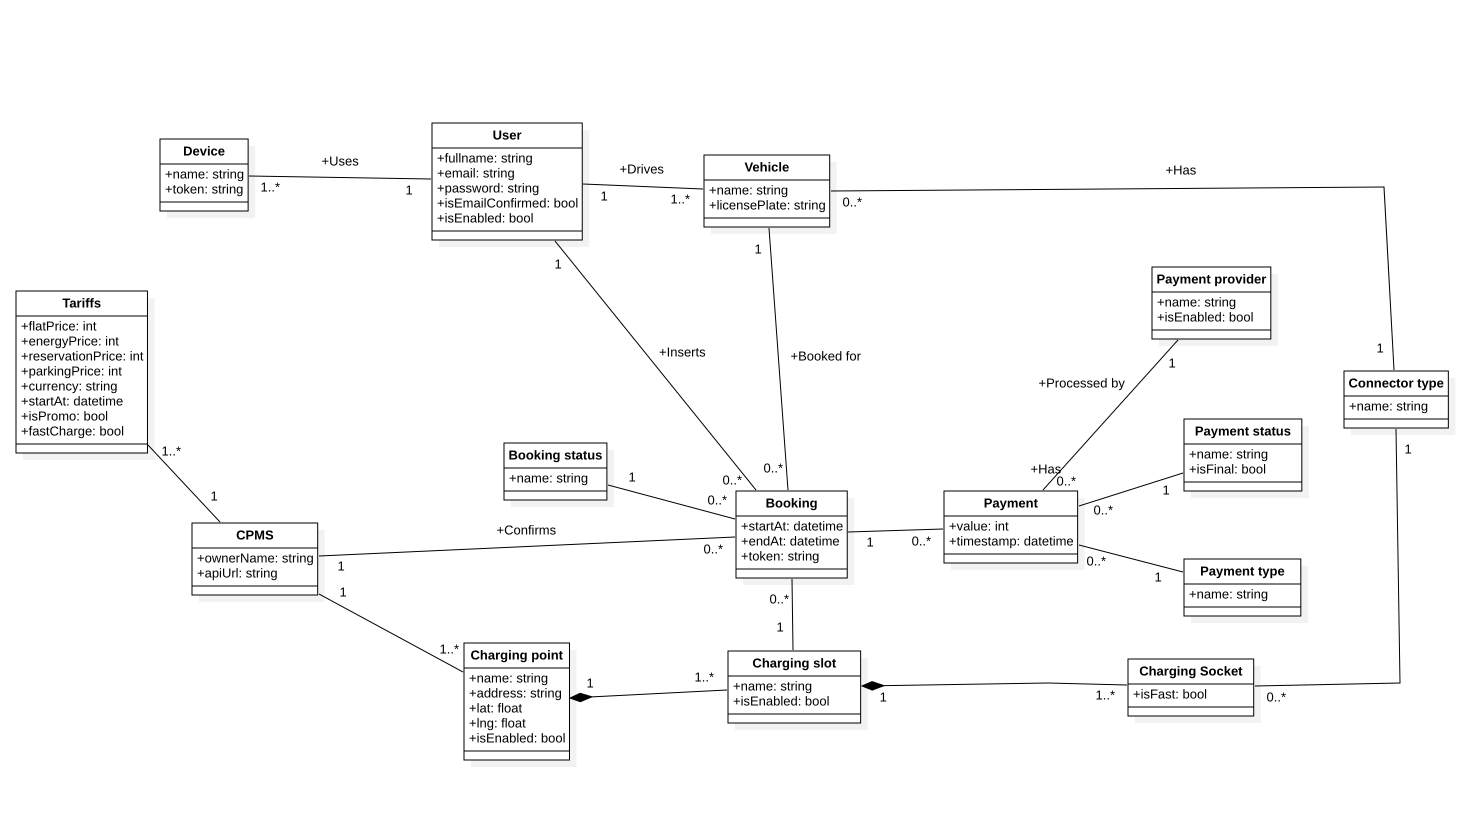
\includegraphics[width=\textwidth]{class_diagram}
\caption{Class diagram of the eMSP system for eMall}
\end{figure}

\clearpage
\newpage

\subsection{State charts}

\begin{figure}[h]
\centering
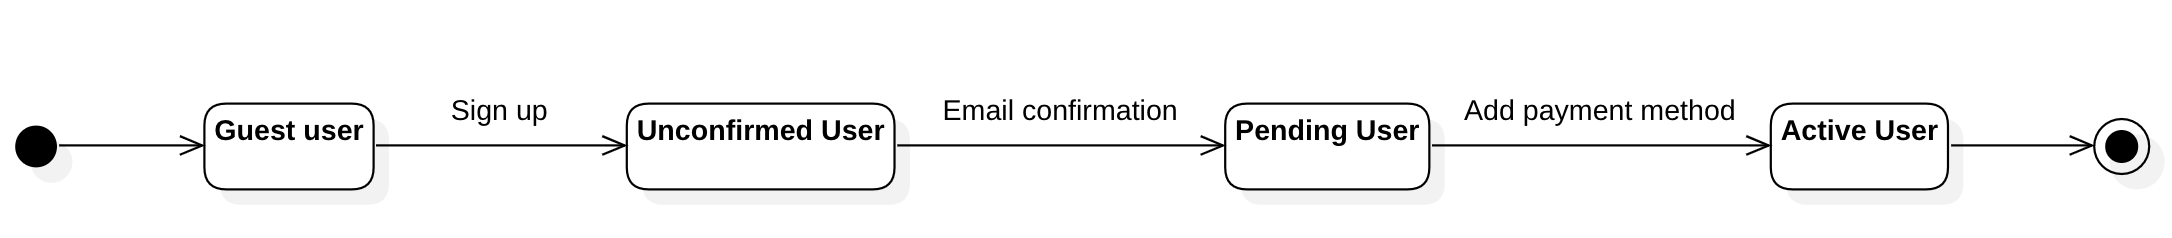
\includegraphics[width=\textwidth]{user_state_diagram}
\caption{State diagram for user registration flow}
\end{figure}

\begin{figure}[h]
\centering
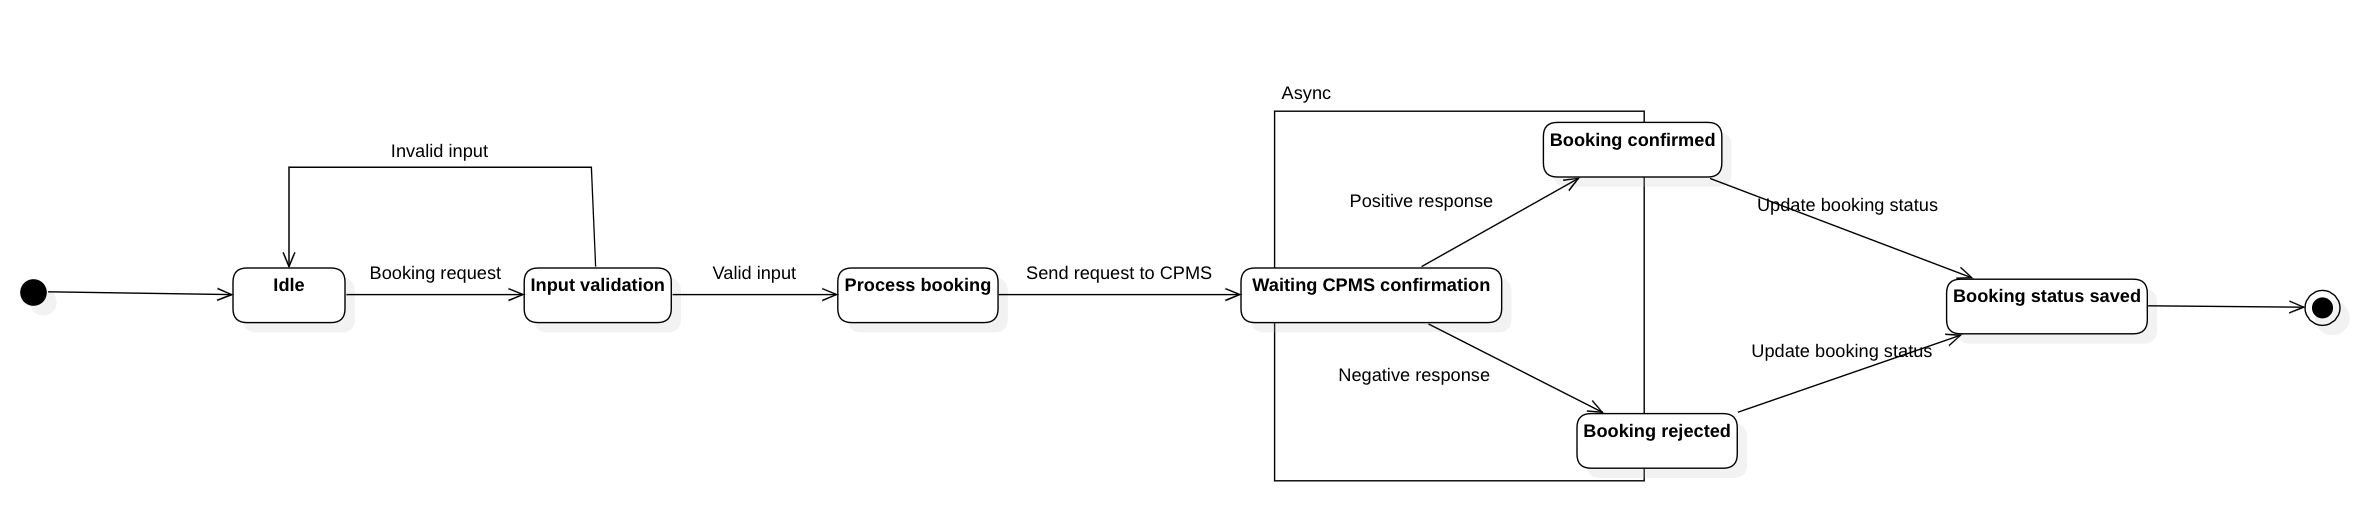
\includegraphics[width=\textwidth]{booking_state_diagram}
\caption{State diagram for Booking}
\end{figure}

\begin{figure}[h]
\centering
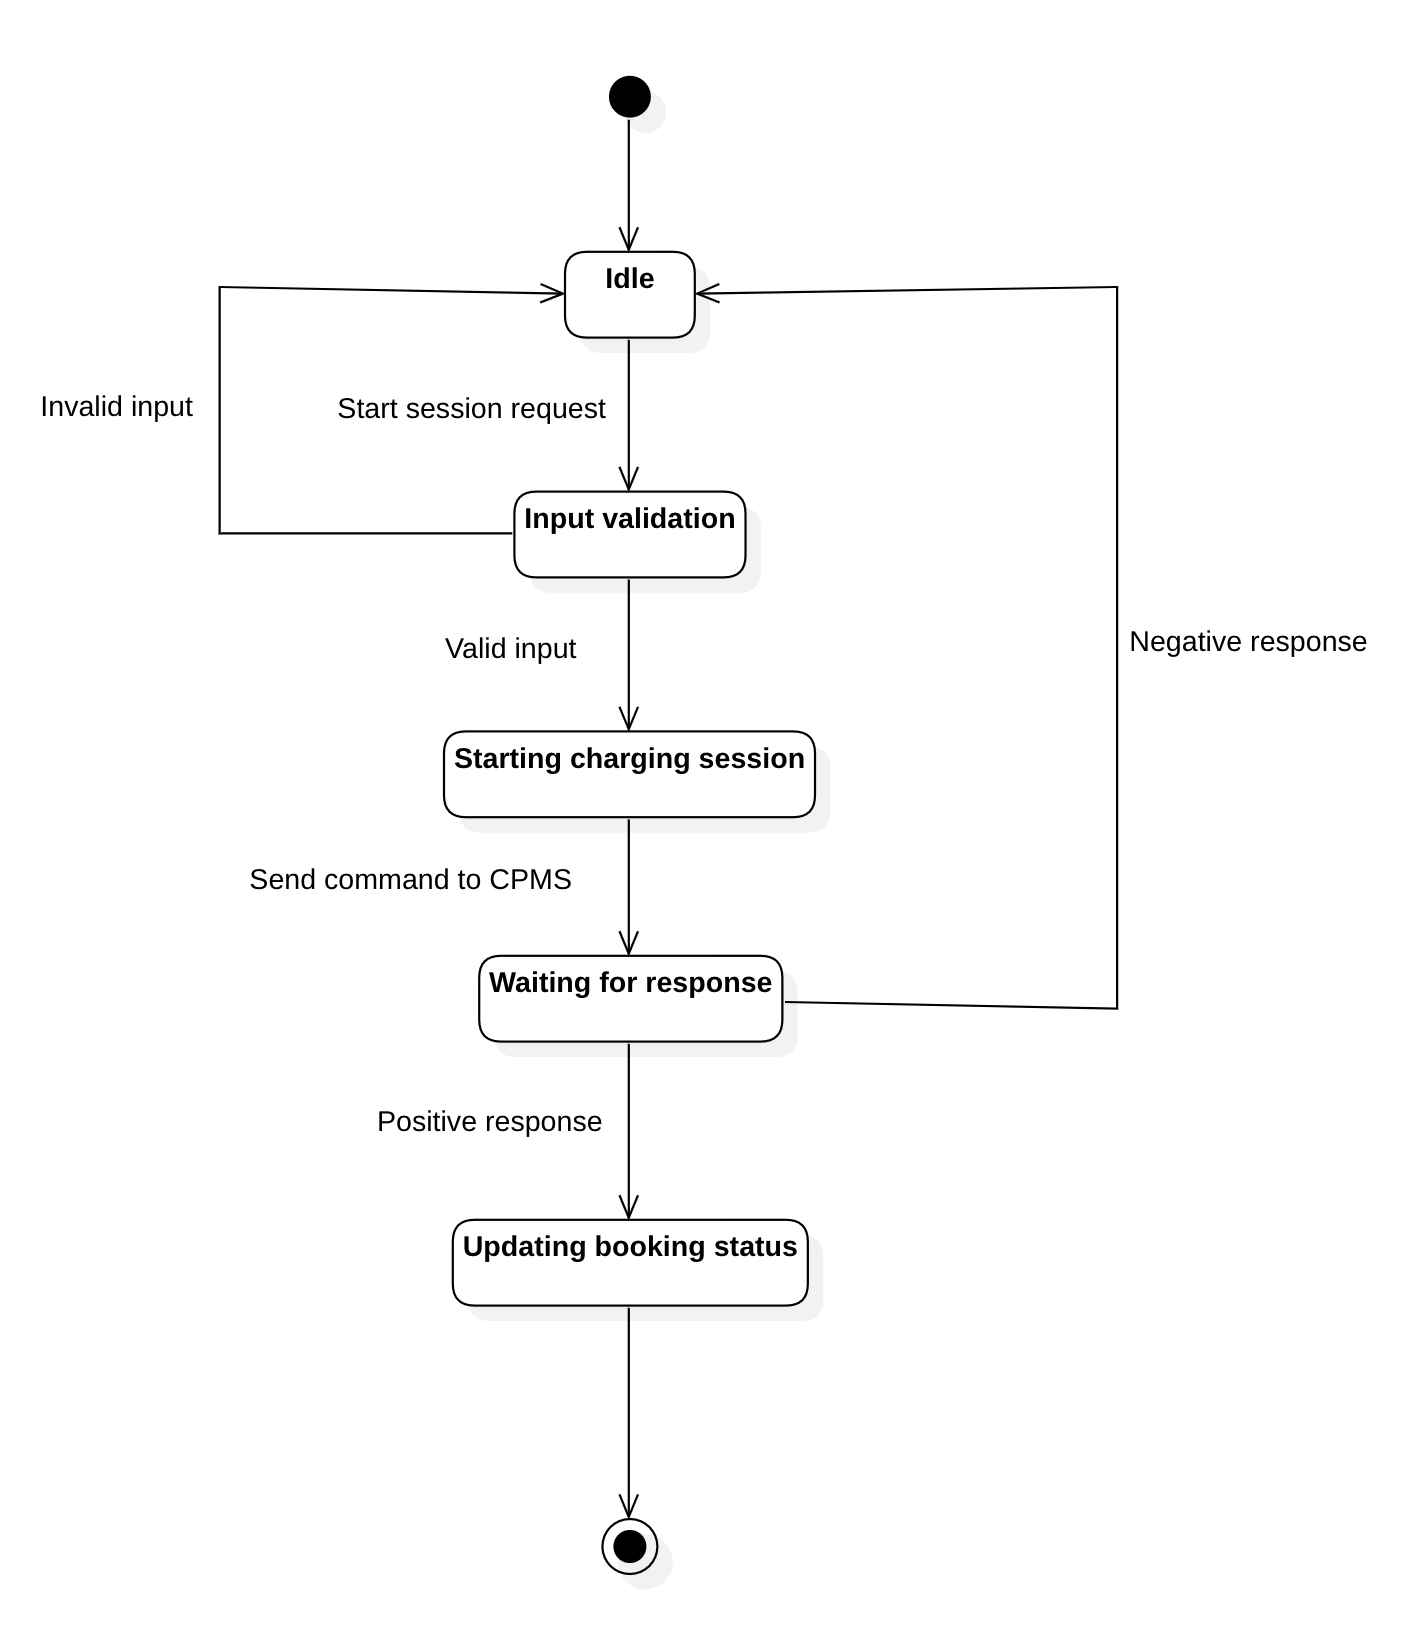
\includegraphics[width=6.2cm]{charging_session_state_diagram}
\caption{State diagram for a Charging Session}
\end{figure}

\clearpage
\newpage


\section{Product functions}
Before going deeply into details about the product functions that needs to be developed and the related requirements, we first need to quickly introduce three base requirements needed to contain the scope of this project:\\

\begin{itemize}
	\item As the system acts as a middleware between the User and the Charging Points, a structured communication protocol is needed. This system will be design to communicate using the Open Charge Point Interface (OCPI) standard.
	\item As OCPI enables a very complex pricing system, to keep the scope of the project simple, the system will use only the per-KW price (also called energy based price), with differentiation between fast charging and non-fast charging. Time limited promotions are also allowed. The prices are synced by the CPMSs via the PUSH interface defined in the OCPI protocol. (i.e. at any time, each CPMS can define only two active prices: standard and fast-charging)
	\item Another limitation that we need to impose to reduce the complexity is the various connector types. We define only two generic types of connector: standard and fast-charging, each type has its own pricing defined by the CPMS.
\end{itemize}

\subsection{Nearby charging points overview}
The users want to quickly find nearby charging points and see their status, the available slots, their connectors and the tariffs, this will allow them to decide where to charge their vehicles or not.\\
To achieve this, the system should act as an aggregator for multiple CPMS, collect the data in real-time and display all the information on a map.

\subsection{Booking a charging slot}
When a user has decided where to charge his vehicle, he can use the same system to book the slot for a specific time frame.\\
As for the OCPI standard booking is managed by the CPMS, the system will need to request booking confirmation from the CPMS.\\
Also OCPI standard allows only reservations that starts at the time of the request so only those type of booking will be considered in the project.

\subsection{Unlocking a charging slot and starting a charge session}
When a user arrives at the charging point he can use the app to review the booking details and check to which slot to connect the vehicle. He connects the car via the correct plug provided by the charging slot and, afterward, he uses the app to authenticate into the system and start charging. Even if OCPI standard allows for other types of session initialisation, our system will not deal with them.

\subsection{Checking the status of the charge session}
After initiating the charge the user will be able to view the status of the session (charge level and estimated time remaining) from the app.\\
The system automatically retrieves (and receives via PUSH) the needed information from the CPMS and eventually notifies the user about any problem that can occur (e.g. charge session is interrupted by the Charge Point Operator)

\subsection{Completing the charge session and paying for the service}
A user can complete the charge session when the charge is completed or even before.\\
To complete a charge session the user can use the app to stop the charging process and detach the plug from the vehicle.\\
As stated above, the payment request is automatically triggered and the payment service provider will charge the user the right amount and send the invoice via email. The complete cost of the service is received with the final status update for the charging session from the CPMS.

\section{User characteristics}
For the scope of the document, we can identify a single user type for the eMall system, but to allow us to better define some details later on, we've split the user based on his possible states

\begin{enumerate}
	\descitem{Unregistered user / guest}
	A person who is not already registered to the system
	
	\descitem{Registered user waiting for email verification}
	A person who is registered to the system but has yet to confirm the email address used in the signup form.
	
	\descitem{Registered user waiting for payment method registration}
	A person who is registered to the system, has his email verified but needs to add a payment method to start using the app.

	\descitem{eMall active user}
	A person who is registered to the system, has a verified email address and an active and valid payment method. Payment method verification is handled by the Payment Service Provider.
	
	\descitem{eMall disabled user}
	An active user that has been flagged for deactivation by the system admin. Could be for security reasons, for direct request from the customer or for terms of service violation.

\end{enumerate}

\section{Assumptions, dependencies and constraints}

\subsection{Assumptions}
\begin{tabular}{|l|l|}
	\hline
	D1 & There is a system admin that does the initial setup of the system and manages it\\
	\hline
	D2 & System admin adds information about CPMS to the database\\
	\hline
	D3 & Users accept the contract and terms of service when signing up into the system\\
	\hline
	D4 & Users always complete their booked charging sessions\\
	\hline
\end{tabular}























\end{document}